\chapter{Distributed Architectural Styles}

\subsection{Service-based Architecture}


\begin{center}
  \begin{minipage}{0.65\linewidth}
    Distributed macro-layered structure: UI+ services

    Quanta: UI separately deployed. Separately deployed coarse-grained services. Optionally, monolithic database

    Domain services are independent,
    usually do not communicate each
    other
  \end{minipage}%
  \hfill
  \begin{minipage}{0.3\linewidth}
    \centering
    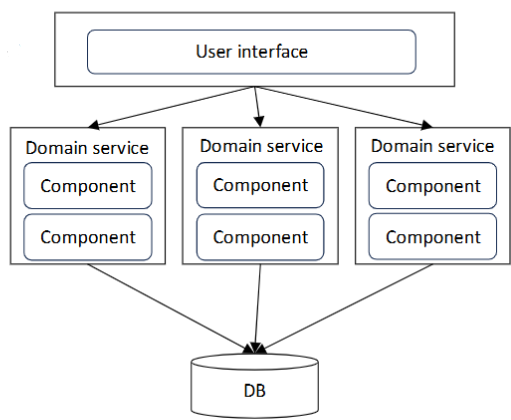
\includegraphics[width=0.5\linewidth]{content/chapters/images/2026-05-20-21-44-33.png}
  \end{minipage}
\end{center}


\subsection{Domain services design}

\begin{figure}[h!]
  \centering
  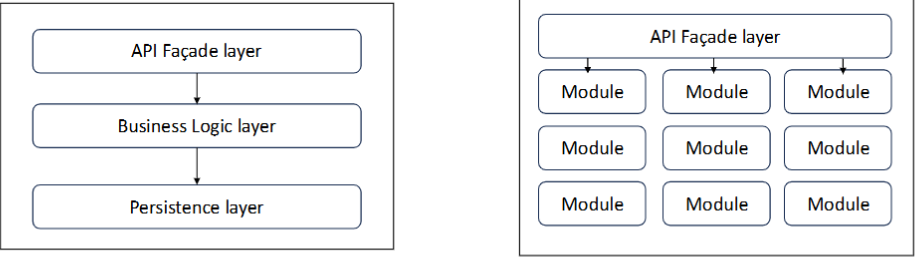
\includegraphics[width=0.3\linewidth]{content/chapters/images/2026-05-20-21-46-29.png}
  \caption{Technical partitioning and Domain partitioning}
\end{figure}

\subsection{API access, UI and DB options}

API access façade acts as orchestrator: failures can be handled at this level.

UI/DB options: Single monolithic, Domain-based or Service-based.

API gateway options between UI and domain services.

\begin{center}
  \begin{minipage}[t]{0.7\linewidth}
  \begin{minipage}[t]{0.45\linewidth}
    \centering
    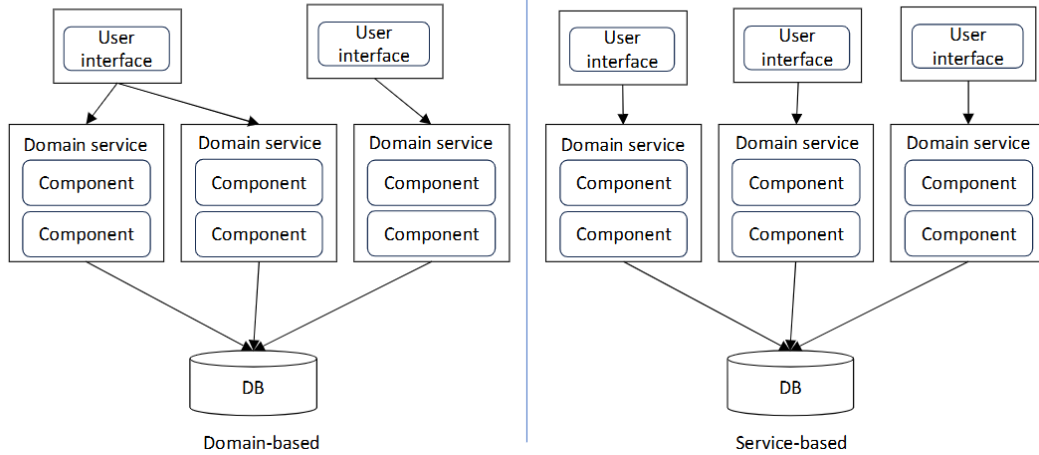
\includegraphics[width=\linewidth]{content/chapters/images/2026-05-20-21-48-20.png}
    \captionof{figure}{UI options}
  \end{minipage}%
  \hfill
  \begin{minipage}[t]{0.45\linewidth}
    \centering
    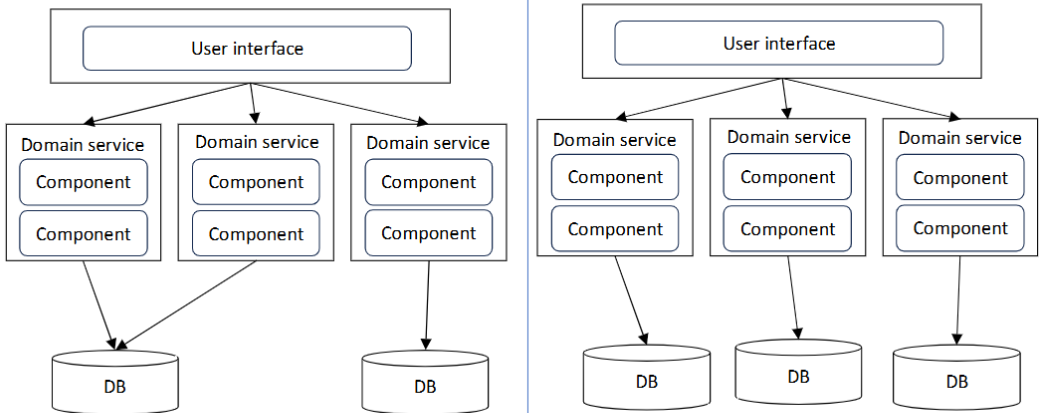
\includegraphics[width=\linewidth]{content/chapters/images/2026-05-20-21-48-30.png}
    \captionof{figure}{DB options}
  \end{minipage}
  \end{minipage}
\end{center}




\subsection{Database logical partitioning}

Using a single shared library for
DB entity objects impacts all
services in cases of changes.
Logical partitioning and multiple
share libraries for db entity
objects reduces coupling.
It should be as fine-grained as
possible

\begin{flushleft}
  \begin{minipage}{0.65\linewidth}
    \raggedright
    Using a single shared library for
    DB entity objects impacts all
    services in cases of changes.
    Logical partitioning and multiple
    share libraries for db entity
    objects reduces coupling.
    It should be as fine-grained as
    possible.

    \paragraph{When to Use}
    \begin{itemize}
      \item Small-medium systems
      \item Limited scalability needs
      \item No or low need of service coordination
      \item Teams new to distributed systems
      \item As intermediate steps towards migration to other distributed styles
    \end{itemize}
  \end{minipage}%
  \hfill
  \begin{minipage}{0.3\linewidth}
    \centering
    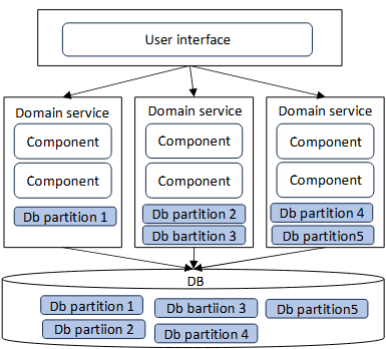
\includegraphics[width=\linewidth]{content/chapters/images/2026-05-21-09-54-08.png}
  \end{minipage}
\end{flushleft}

\subsection{Service-based architecture: characteristics}

\begin{table}[h!]
  \renewcommand{\arraystretch}{1.4}
  \centering
  \begin{tabularx}{\textwidth}{l X l X}
    \toprule
     & \textbf{Characteristic} & \textbf{Rating} & \textbf{Notes}                               \\
    \midrule
    \multirow{2}{*}{Structural}
     & Simplicity              & Medium          &                                              \\
     & Modularity              & Medium          & Domain scoping, federated UI and BD possible \\
    \midrule
    \multirow{4}{*}{Engineering}
     & Maintainability         & High            & As consequence of modularity                 \\
     & Testability             & High            & As above                                     \\
     & Deployability           & High            & As above                                     \\
     & Evolvability            & High            & As above                                     \\
    \midrule
    \multirow{4}{*}{Operational}
     & Responsiveness          & Medium          &                                              \\
     & Scalability             & Medium          & Coarse-grained services                      \\
     & Elasticity              & Low             &                                              \\
     & Fault tolerance         & Medium          & Self-contained services                      \\
    \bottomrule
  \end{tabularx}
\end{table}

\section{Microservices architecture}

Domain partitioning took to the extreme.
Heavily inspired by the idea of domain-driven-design and DevOps


Fundamental concept of ``bounded context''

\begin{itemize}
  \item Everything related to a portion of the domain is visible internally but
        opaque to other bounded contexts
  \item It drives systematically interventions of decoupling
\end{itemize}

Protocol-aware heterogenous interoperability
\begin{itemize}
  \item Standardized communications (e.g., REST)
  \item Independent services
  \item Inter-service communication possible
\end{itemize}


\begin{center}
  \begin{minipage}{0.6\linewidth}
    \begin{minipage}{0.47\linewidth}
      \centering
      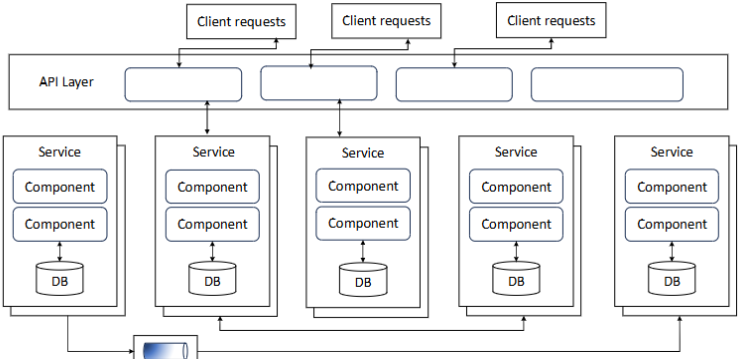
\includegraphics[width=\linewidth]{content/chapters/images/2026-05-21-10-12-28.png}
      \captionof{figure}{Overview}
    \end{minipage}%
    \hfill
    \begin{minipage}{0.47\linewidth}
      \centering
      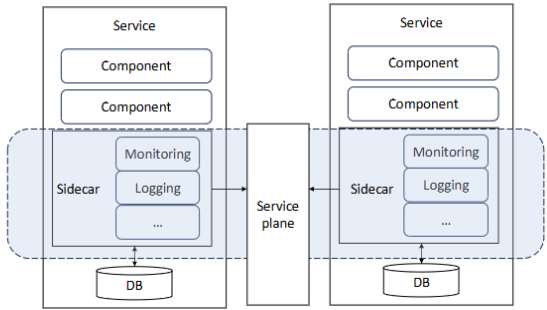
\includegraphics[width=\linewidth]{content/chapters/images/2026-05-21-10-12-40.png}
      \captionof{figure}{Monitoring and governance: sidecar pattern}
    \end{minipage}
  \end{minipage}
\end{center}

\subsection{Granularity of services}


Extreme granularity may affect performances

Main decision criteria for micro-services:
\begin{itemize}
  \item Purpose (i.e., problem domain)
  \item (Avoid/minimize) transactions
  \item Choreography
\end{itemize}

Other aspects:
\begin{itemize}
  \item Data isolation: per service or per domain
  \item API layer ``neutrality''
  \item Frontends: monolithic vs coupling with backend services
  \item Choreography vs orchestration
\end{itemize}


\subsection{Microservices architecture: characteristics}

\begin{table}[h!]
  \renewcommand{\arraystretch}{1.4}
  \centering
  \begin{tabularx}{\textwidth}{l X l X}
    \toprule
     & \textbf{Characteristic} & \textbf{Rating} & \textbf{Notes}                                                                                  \\
    \midrule
    \multirow{2}{*}{Structural}
     & Simplicity              & Very low        &                                                                                                 \\
     & Modularity              & Very high       &                                                                                                 \\
    \midrule
    \multirow{4}{*}{Engineering}
     & Maintainability         & Very high       &                                                                                                 \\
     & Testability             & Very high       &                                                                                                 \\
     & Deployability           & Very high       &                                                                                                 \\
     & Evolvability            & Very high       &                                                                                                 \\
    \midrule
    \multirow{4}{*}{Operational}
     & Responsiveness          & Low             & Many network calls to complete work; data caching and replication + choreography can improve it \\
     & Scalability             & Very high       &                                                                                                 \\
     & Elasticity              & High            &                                                                                                 \\
     & Fault tolerance         & Very high       &                                                                                                 \\
    \bottomrule
  \end{tabularx}
\end{table}

\section{Event-driven architecture}

Main implementation: choreographed and technically partitioned
Decoupled event processing components asynchronously trigger and
responds via events. Asynchronous fire-and-forget communication. Loose coupling.

Four primary components:
\begin{itemize}
  \item Initiating event
  \item Event broker
  \item Event processor
  \item Derived events
\end{itemize}

\begin{center}
  \begin{minipage}{0.7\linewidth}
    \begin{minipage}{0.45\linewidth}
      \centering
      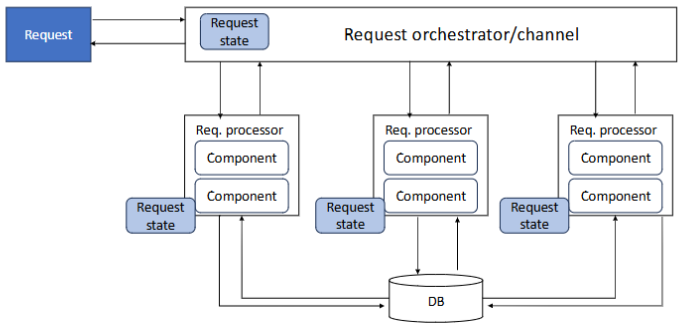
\includegraphics[width=\linewidth]{content/chapters/images/2026-05-21-10-21-35.png}
      \captionof{figure}{Event-driven architecture}
    \end{minipage}%
    \hfill
    \begin{minipage}{0.45\linewidth}
      \centering
      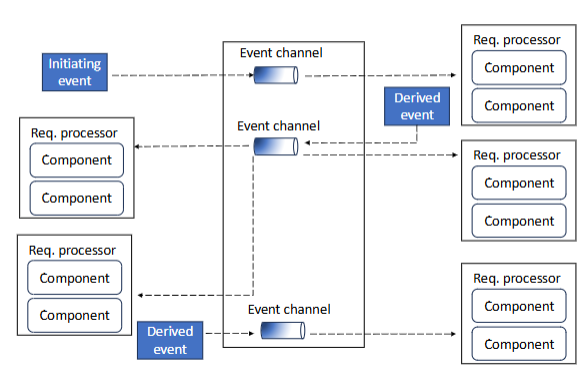
\includegraphics[width=\linewidth]{content/chapters/images/2026-05-21-10-21-55.png}
      \captionof{figure}{Fire and forget}
    \end{minipage}
  \end{minipage}
\end{center}

\paragraph{EDA processing - example with SPG}

\begin{figure}[h!]
  \centering
  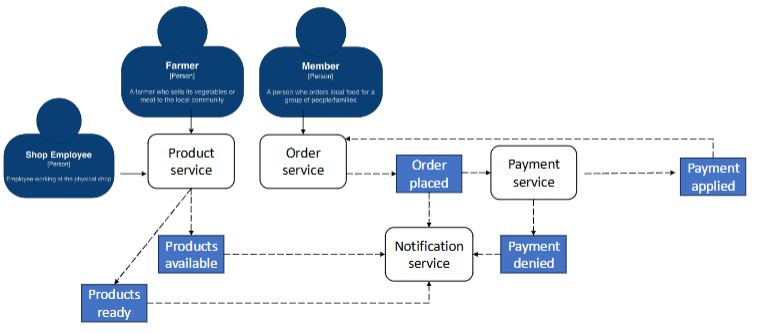
\includegraphics[width=0.3\linewidth]{content/chapters/images/2026-05-21-10-23-04.png}
\end{figure}

\subsection{Events vs messages}

\begin{table}[h!]
  \renewcommand{\arraystretch}{1.4}
  \centering
  \begin{tabularx}{\textwidth}{>{\bfseries\centering\arraybackslash}X >{\centering\arraybackslash}X >{\centering\arraybackslash}X}
    \toprule
                          & \textbf{EVENTS}                           & \textbf{MESSAGES}                                         \\
    \midrule
    ACTION                & Reacting to something already happened    & Obeying to a request with something that needs to be done \\
    \midrule
    ANSWER                & It doesn't require an answer              & It -typically- requires an answer                         \\
    \midrule
    COMMUNICATION STYLE   & One-to-many (e.g., publish and subscribe) & One-to-one (or point-to-point)                            \\
    \midrule
    COMMUNICATION CHANNEL & Topic, stream, notification service       & Queue, messaging service                                  \\
    \bottomrule
  \end{tabularx}
\end{table}

\subsection{Further options}

\begin{itemize}
  \item \textbf{Triggering extensible events}: It increases evolvability of the systems
  \item \textbf{Asynchronous vs synchronous = performance vs responsiveness}: NB asynchronous communication decouples architectural quanta
  \item Broadcast capabilities for implementing semantic decoupling
  \item Granularity of events: Be aware of swarm of gnats antipattern !
  \item Error handling through Workflow Event pattern or tools
\end{itemize}

\subsection{Event payload}

\begin{flushleft}
  \begin{minipage}[t]{0.45\linewidth}
    \paragraph{Data-based payload}
    \raggedright

    \begin{itemize}
      \item It avoids pression on DB: payload contains all information for
            subscribers
      \item Extra support for data consistency and integrity
      \item Data format creates coupling: Stamp coupling
      \item Versioning: Data and Contract
    \end{itemize}

  \end{minipage}%
  \hfill
  \begin{minipage}[t]{0.45\linewidth}
    \paragraph{Key-based payload}
    \raggedright
    \begin{itemize}
      \item Payload contains pairs of keyvalues to later query a DB.
            Typically, JSON or XML,  Human readable

      \item DB remains the single source of
            information
      \item Minimum contracts and network
            usage
      \item No need of versioning
    \end{itemize}

  \end{minipage}
\end{flushleft}

\paragraph{Event payload - Example}

\begin{figure}[h!]
  \centering
  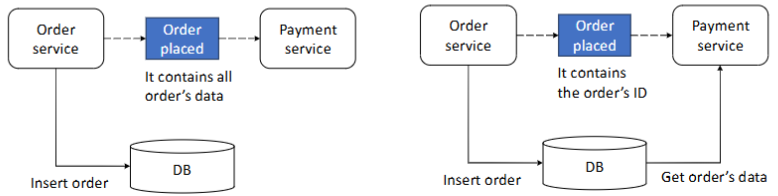
\includegraphics[width=0.4\linewidth]{content/chapters/images/2026-05-21-10-31-40.png}
  \caption{Data-based payload, Key-based payload }
\end{figure}

\subsection{Events payload: tradeoffs}

\begin{table}[h!]
  \renewcommand{\arraystretch}{1.4}
  \centering

  % Definizione rapida delle icone colorate
  \newcommand{\good}{\textcolor{green!60!black}{\smiley}}
  \newcommand{\bad}{\textcolor{red!80!black}{\frownie}}

  \begin{tabularx}{\textwidth}{>{\bfseries}X >{\centering\arraybackslash}X >{\centering\arraybackslash}X}
    \toprule
                                & \textbf{DATA-BASED} & \textbf{KEY-BASED} \\
    \midrule
    Performance and scalability & \good               & \bad               \\
    Contract management         & \bad                & \good              \\
    Stamp coupling              & \bad                & \good              \\
    Bandwidth utilization       & \bad                & \good              \\
    Restricted db access        & \good               & \bad               \\
    Overall system fragility    & \bad                & \good              \\
    \bottomrule
  \end{tabularx}
\end{table}


\subsection{Data loss prevention}

\begin{enumerate}
  \item While A publishes an event, it crashes before ack from event broker
  \item B accepts an event, but it crashes before processing it
  \item A data error prevents B from ensuring persistence
\end{enumerate}


\begin{figure}[h!]
  \centering
  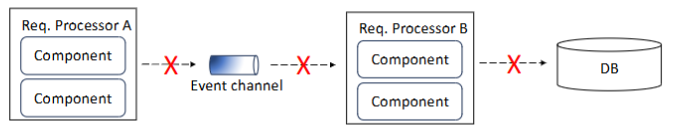
\includegraphics[width=0.3\linewidth]{content/chapters/images/2026-05-21-10-34-54.png}
  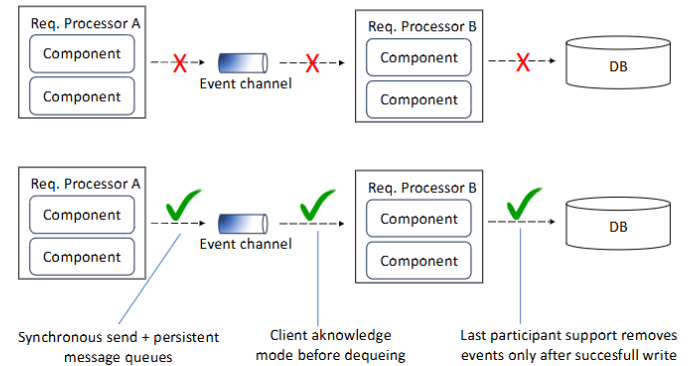
\includegraphics[width=0.25\linewidth]{content/chapters/images/2026-05-21-10-35-27.png}
\end{figure}


\subsection{Request-reply processing}
Also known as \textit{pseudosynchronous communications}.
It requires a request queue and a reply queue.
Event producers waits until confirmation of event producer is
retrieved fomr the reply queue.

Two common implementations:
\begin{itemize}
  \item Correlation ID
  \item Temporary queue with specific id
\end{itemize}

\section{Orchestrated EDA}


\begin{center}
  \begin{minipage}{0.65\linewidth}
    Orchestration vs Choreography.

    Mediation by a specific component/service.

    Event mediator typically uses messages.
    The mediator is responsible of catching events and generate specific
    point-to-point derivated events. Usually with queues. Without further communicating its own actions (fire and forget principle)


    Orhestrator's options: monolithic, domain-based, service-dedicated.
  \end{minipage}%
  \hfill
  \begin{minipage}{0.3\linewidth}
    \centering
    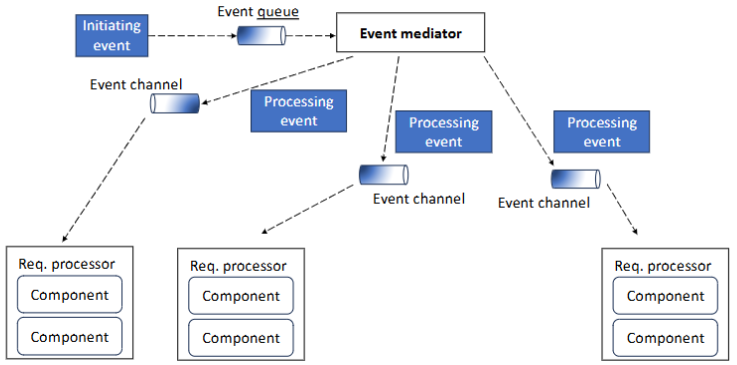
\includegraphics[width=\linewidth]{content/chapters/images/2026-05-21-10-38-58.png}
  \end{minipage}
\end{center}

\subsection{Event drive architecture: usage}

\begin{flushleft}
  \begin{minipage}[t]{0.45\linewidth}
    \raggedright

    \paragraph{When to use}

    \begin{itemize}
      \item Complex workflows, with thousands scenarios
      \item Dynamic user content
      \item Reactive systems
      \item Real time processing
    \end{itemize}
  \end{minipage}%
  \hfill
  \begin{minipage}[t]{0.45\linewidth}
    \raggedright

    \paragraph{When NOT to use}

    \begin{itemize}
      \item High needs of synchronous communication
      \item Static coupling (contracts) increases
      \item Dynamic coupling (sync calls) increases
    \end{itemize}
  \end{minipage}
\end{flushleft}


\subsection{EDA architecture: characteristics}

\begin{table}[h!]
  \renewcommand{\arraystretch}{1.4}
  \centering
  \begin{tabularx}{\textwidth}{l l l X}
    \toprule
    \textbf{}   & \textbf{Characteristic} & \textbf{Rating} & \textbf{Notes}                                          \\
    \midrule
    Structural  & Simplicity              & Low             & Dependent also on dynamic coupling and data topologies  \\
                & Modularity              & High            &                                                         \\
    \midrule
    Engineering & Maintainability         & High            &                                                         \\
                & Testability             & Low             & Due to non-deterministic workflow                       \\
                & Deployability           & Medium          &                                                         \\
                & Evolvability            & Very high       &                                                         \\
    \midrule
    Operational & Responsiveness          & Very high       &                                                         \\
                & Scalability             & High            & Additional processors can be added; db still bottleneck \\
                & Elasticity              & Medium          &                                                         \\
                & Fault tolerance         & Very high       &                                                         \\
    \bottomrule
  \end{tabularx}
\end{table}

\section{Space-based architecture}




\begin{flushleft}
  \begin{minipage}{0.65\linewidth}
    \raggedright
    Technically partitioned. Complex implementation. Designed to optimize operations with large volumes of data, users,
    and load peaks.


    Main features:
    \begin{itemize}
      \item Eliminates database bottleneck
      \item Distributed data management
      \item Distributed processing units
    \end{itemize}
  \end{minipage}%
  \hfill
  \begin{minipage}{0.3\linewidth}
    \centering
    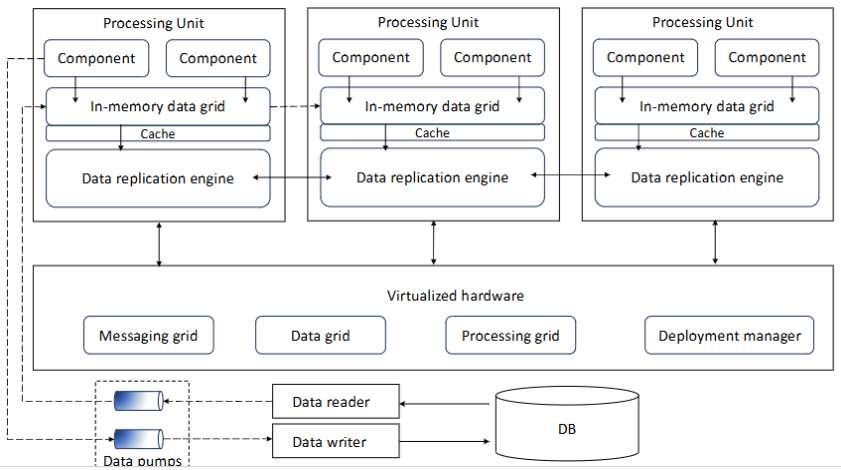
\includegraphics[width=\linewidth]{content/chapters/images/2026-05-21-10-42-58.png}
  \end{minipage}
\end{flushleft}


\subsection{Space-based architecture: elements}

\begin{table}[h!]
  \renewcommand{\arraystretch}{1.4}
  \centering
  \begin{tabularx}{\textwidth}{l X}
    \toprule
    \textbf{Element name}  & \textbf{Description}                                                                                                                                                  \\
    \midrule
    Processing units       & Contain the application functionality                                                                                                                                 \\
    Virtualized middleware & The collection of infrastructure-related artifacts that are used to manage and coordinate the processing units                                                        \\
    Messaging grid         & It manages input requests and session states (e.g., a web server with load balancing)                                                                                 \\
    Data grid              & Manages the synchronization and replication of data between processing units. It can be implemented also in processing units.                                         \\
    Processing grid        & Used to manage request orchestration between multiple processing units; optional                                                                                      \\
    Deployment manager     & Manages the starting and tearing down of processing unit instances based on load                                                                                      \\
    Data pumps             & Asynchronously send updated data to the database. It decouples processing units and database. Usually implemented with messaging and queues. Can be mapped to domains \\
    Data writers           & Perform the updates from the data pumps. They can be multiple and dedicated to data pumps                                                                             \\
    Data readers           & Read database data and deliver it to processing units (upon startup) through reverse data pumps.                                                                      \\
    \bottomrule
  \end{tabularx}
\end{table}

\subsection{Replicated cache data: collisions}

Collisions typically occur when the update rate of the data in the
cache exceeeds the replication latency.

Several factors influence the amount of data collisions:

\begin{itemize}
  \item N : \# of processing unit instances containing the same cachce
  \item UR: cache update rate (updates/seconds)
  \item S: cache size (\# of rows)
  \item RL: Replication latency (milliseconds)
\end{itemize}

\begin{equation*}
  \text{Collision Rate} = N \times \frac{UR^2}{S} \times RL
\end{equation*}

\subsection{Distributed caching}

\begin{figure}[h!]
  \centering
  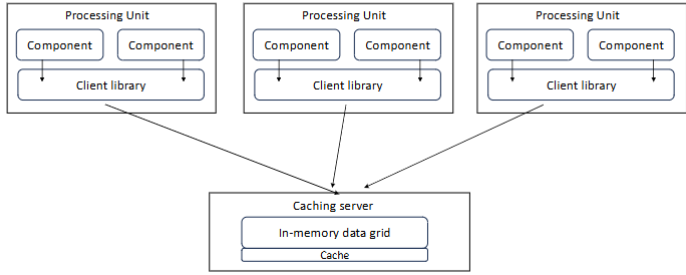
\includegraphics[width=0.3\linewidth]{content/chapters/images/2026-05-21-14-02-54.png}
\end{figure}

\subsection{Replicated vs distributed caching}
= Asynchronous replication vs synchronous replication
Replicated caching:

\begin{itemize}
  \item requires in-memory data grid, very fast
  \item difficult with very high data volumes and frequent updates
  \item possible also wih near-cache techniques: a caching server + partial front caches
\end{itemize}

\begin{table}[h!]
  \renewcommand{\arraystretch}{1.4}
  \centering
  \begin{tabularx}{\textwidth}{X X}
    \toprule
    \textbf{} & \textbf{} \\
    \midrule
              &           \\
              &           \\
              &           \\
              &           \\
              &           \\
    \bottomrule
  \end{tabularx}
\end{table}

\section{SBA architecture - Usage}

\begin{table}[h!]
  \renewcommand{\arraystretch}{1.4}
  \centering
  \begin{tabularx}{\textwidth}{X X X}
    \toprule
    \textbf{Criteria} & \textbf{Replicated} & \textbf{Distributed} \\
    \midrule
    Optimization      & Performance         & Consistency          \\
    Cache size        & Small               & Large                \\
    Type of data      & Mostly static       & Highly dynamic       \\
    Update frequency  & Low                 & High                 \\
    Fault tolerance   & High                & Low                  \\
    \bottomrule
  \end{tabularx}
\end{table}


\subsection{When to use:}

\begin{itemize}
  \item High volume applications
  \item Large, concurrent user load
  \item Low-latency systems
\end{itemize}


\subsection{Space based architecture: characteristics}

\begin{table}[h!]
  \renewcommand{\arraystretch}{1.4}
  \centering
  \begin{tabularx}{\textwidth}{l l l X}
    \toprule
    \textbf{}   & \textbf{Characteristic} & \textbf{Rating} & \textbf{Notes}                                                     \\
    \midrule
    Structural  & Simplicity              & Very low        &                                                                    \\
                & Modularity              & Medium          & Technically partitioned                                            \\
    \midrule
    Engineering & Maintainability         & Medium          &                                                                    \\
                & Testability             & Very low        & Difficult to simulate very high loads                              \\
                & Deployability           & Medium          &                                                                    \\
                & Evolvability            & Medium          &                                                                    \\
    \midrule
    Operational & Responsiveness          & Very high       &                                                                    \\
                & Scalability             & Very high       &                                                                    \\
                & Elasticity              & Very high       &                                                                    \\
                & Fault tolerance         & Low             & Technically partitioned, distributed computing and data management \\
    \bottomrule
  \end{tabularx}
\end{table}



\section{Orchestration-driven service-oriented architecture}

\begin{flushleft}
  \begin{minipage}{0.65\linewidth}
    \raggedright
    \begin{itemize}
      \item Enterprise-level architecture
      \item Layers with specific responsibilities
      \item Strong governance through taxonomy of services
      \item Services share enterprise bus
      \item Usage in companiesdecreasing, due to extreme technical partitioning
    \end{itemize}
  \end{minipage}%
  \hfill
  \begin{minipage}{0.3\linewidth}
    \centering
    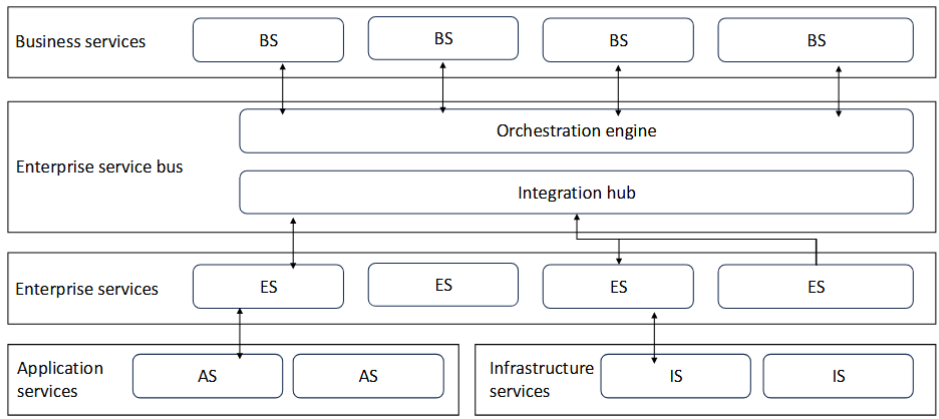
\includegraphics[width=\linewidth]{content/chapters/images/2026-05-23-12-43-49.png}
  \end{minipage}
\end{flushleft}

\subsection{Service-oriented architecture: layers}





\begin{flushleft}
  \begin{minipage}{0.65\linewidth}
    \raggedright
    \begin{itemize}
      \item \textbf{Business services:} no business logic, no code, only I/O schemas (service signatures)
      \item \textbf{Entrerprise service bus:} Transaction coordination and message transformation. Also for internal calls, it can “eat” the whole architecture
      \item \textbf{Enterprese services:} Building blocks of isolated and combinable/reusable functionalities
      \item \textbf{Application services:} one-off, single implementation services, typically not reusable
      \item \textbf{Infrastracture services:} Monitoring, authentication, logging
    \end{itemize}

    \paragraph{Reasons for decay after the 2010s}
    Domains concepts spread so thinely
    that they were virtually ground to
    dust
  \end{minipage}%
  \hfill
  \begin{minipage}{0.3\linewidth}
    \centering

    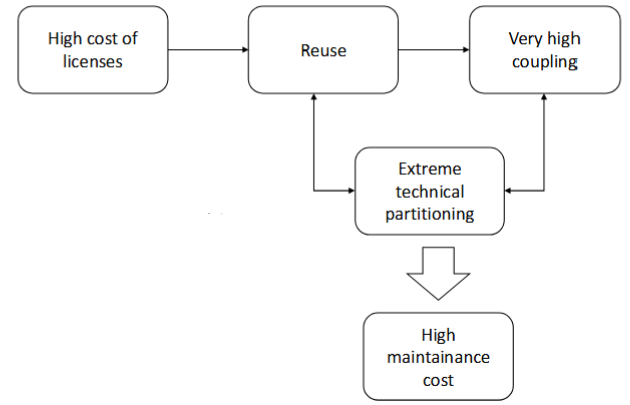
\includegraphics[width=\linewidth]{content/chapters/images/2026-05-23-12-50-08.png}
  \end{minipage}
\end{flushleft}


\subsection{ODSA architecture: characteristics}

\begin{table}[h!]
  \renewcommand{\arraystretch}{1.4}
  \centering
  \begin{tabularx}{\textwidth}{l l l X}
    \toprule
    \textbf{}   & \textbf{Characteristic} & \textbf{Rating} & \textbf{Notes}                                  \\
    \midrule
    Structural  & Simplicity              & Very low        &                                                 \\
                & Modularity              & High            &                                                 \\
    \midrule
    Engineering & Maintainability         & Very low        & Because of very high coupling                   \\
                & Testability             & Very low        & As above                                        \\
                & Deployability           & Very low        &                                                 \\
                & Evolvability            & Very low        & Ripple effects for any functional/domain change \\
    \midrule
    Operational & Responsiveness          & LOW             &                                                 \\
                & Scalability             & High            & Through session duplication                     \\
                & Elasticity              & Medium          &                                                 \\
                & Fault tolerance         & Medium          &                                                 \\
    \bottomrule
  \end{tabularx}
\end{table}

\section{Distributed Styles Architectural Characteristics: synopsis}


\subsection{Structural and engineering characteristics}

\begin{table}[h!]
  \renewcommand{\arraystretch}{1.4}
  \centering
  \begin{tabularx}{\textwidth}{l l X X X X X}
    \toprule
     & \textbf{Characteristic} & \textbf{Service based} & \textbf{Microservice} & \textbf{Event driven} & \textbf{Space based} & \textbf{Orch. Driven Service or.} \\
    \midrule
    \multirow{2}{*}{Structural}
     & Simplicity              & Very low               & Very low              & Low                   & Very low             & Very low                          \\
     & Modularity              & Very high              & Very high             & High                  & Medium               & High                              \\
    \midrule
    \multirow{4}{*}{Engineering}
     & Maintainability         & Very high              & Very high             & High                  & Medium               & Very low                          \\
     & Testability             & Very high              & Very high             & Low                   & Very low             & Very low                          \\
     & Deployability           & Very high              & Very high             & Medium                & Medium               & Very low                          \\
     & Evolvability            & Very high              & Very high             & Very high             & Medium               & Very low                          \\
    \bottomrule
  \end{tabularx}
\end{table}

\subsection{Operational characteristics}

\begin{table}[h!]
  \renewcommand{\arraystretch}{1.4}
  \centering
  \begin{tabularx}{\textwidth}{l l X X X X X}
    \toprule
     & \textbf{Characteristic} & \textbf{Service based} & \textbf{Microservice} & \textbf{Event driven} & \textbf{Space based} & \textbf{Orch. Driven Service or.} \\
    \midrule
    \multirow{4}{*}{Operational}
     & Responsiveness          & Medium                 & Low                   & Very high             & Very high            & Low                               \\
     & Scalability             & Medium                 & Very high             & High                  & Very high            & High                              \\
     & Elasticity              & Low                    & High                  & Medium                & Very high            & Medium                            \\
     & Fault tolerance         & Medium                 & Very high             & Very high             & Low                  & Medium                            \\
    \bottomrule
  \end{tabularx}
\end{table}



























